\documentclass[a4paper,11pt,BCOR10mm,oneside,headsepline]{scrartcl}
\usepackage{amsmath, mathtools}
\usepackage[ngerman]{babel}
\usepackage[utf8]{inputenc}

\usepackage{typearea, url}
\areaset{17cm}{26cm}
\setlength{\topmargin}{-1cm}
\usepackage{scrpage2}
\pagestyle{scrheadings}

\usepackage[T1]{fontenc}
\usepackage{beramono}
\usepackage{listings}
\usepackage[usenames,dvipsnames]{xcolor}
\usepackage{graphicx}
\usepackage{subcaption}

\ihead{HW3: CIS 631, Parallel Processing}
\ohead{\pagemark}
\chead{}
\cfoot{}

\begin{document}
	
	\begin{center}
		\textbf{\large Homework 3 Report}
	\end{center}\vskip1em
	
	\section{Test Environment}
	I tested my code on department's ix server. It has two sockets with AMD Opteron 6376 on each socket. Each CPU has 8 cores, 16 threads. So, there are 32 hardware threads in total.
	
	\section{Test Results}
	\subsection{Results over 10 runs: Execution Time (seconds)}
		\begin{figure}[!htbp]
			\begin{subfigure}{.5\textwidth}
				\centering
				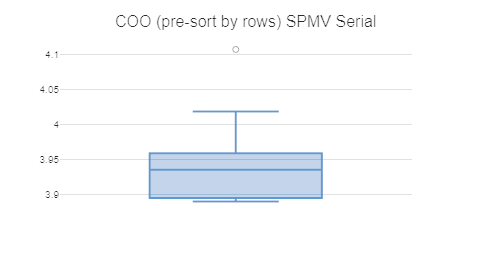
\includegraphics[scale = 0.5]{./figures/coo_serial}
				\caption{Average: 3.9490364}
			\end{subfigure}
			\begin{subfigure}{.5\textwidth}
				\centering
				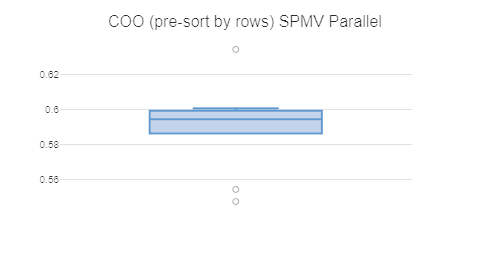
\includegraphics[scale = 0.5]{./figures/coo_parallel}
				\caption{Average: 0.5898402}
			\end{subfigure}
		\end{figure}
	
		\begin{figure}[!htbp]
			\begin{subfigure}{.5\textwidth}
				\centering
				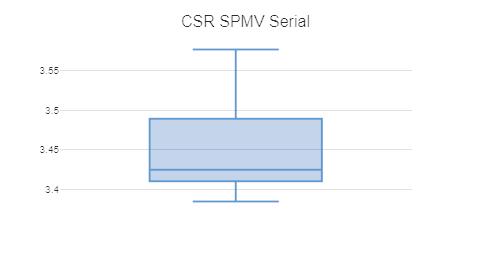
\includegraphics[scale = 0.5]{./figures/csr_serial}
				\caption{Average: 3.4472758}
			\end{subfigure}
			\begin{subfigure}{.5\textwidth}
				\centering
				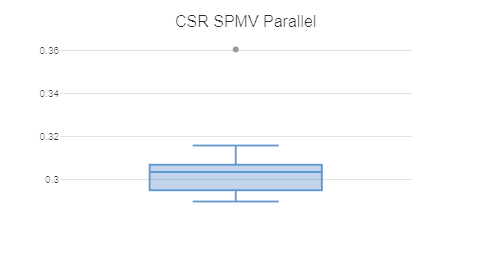
\includegraphics[scale = 0.5]{./figures/csr_parallel}
				\caption{Average: 0.3070956}
			\end{subfigure}
		\end{figure}
	
	\subsection{Performance: COO (pre-sort by rows) vs. CSR}
		\begin{figure}[!htbp]
			\centering
			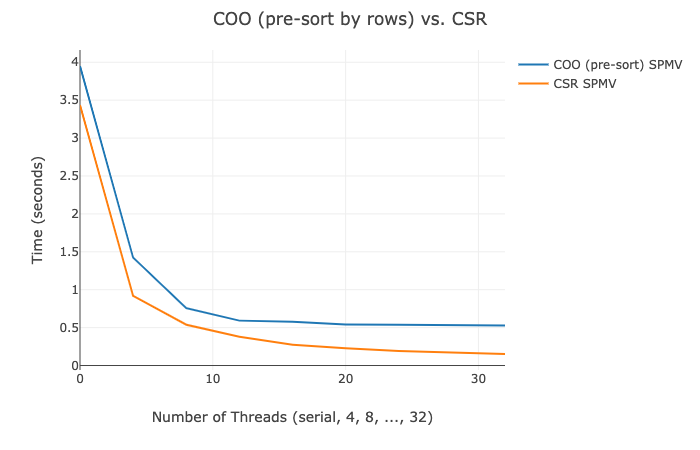
\includegraphics[scale=0.45]{./figures/coo_vs_csr}
		\end{figure}
	
	\subsection{Accuracy (diff results): COO vs. CSR}
	\begin{table}[!htbp]
		\centering
		\begin{tabular}{|c|c|l|l|l|l|l|l|l|l|}
			\hline
			& 0 & 4 & 8 & 12 & 16 & 20 & 24                                                                                               & 28                                                                                               & 32                                                                                                                                                            \\ \hline
			COO & - & - & - & -  & -  & -  & \begin{tabular}[c]{@{}l@{}}\textless 3266.0819162971\\ \textgreater 3266.0819162970\end{tabular} & \begin{tabular}[c]{@{}l@{}}\textless 1271.8511032950\\ \textgreater 1271.8511032951\end{tabular} & \begin{tabular}[c]{@{}l@{}}\textless -4759.7834986281\\ \textgreater -4759.7834986282\\ \textless 2964.0054889568\\ \textgreater 2964.0054889569\end{tabular} \\ \hline
			CSR & - & - & - & -  & -  & -  & -                                                                                                & -                                                                                                & -                                                                                                                                                             \\ \hline
		\end{tabular}
	\end{table}
	
	\subsection{COO: With Pre-Sort vs. Without Pre-Sort}
		\begin{figure}[!htbp]
			\centering
			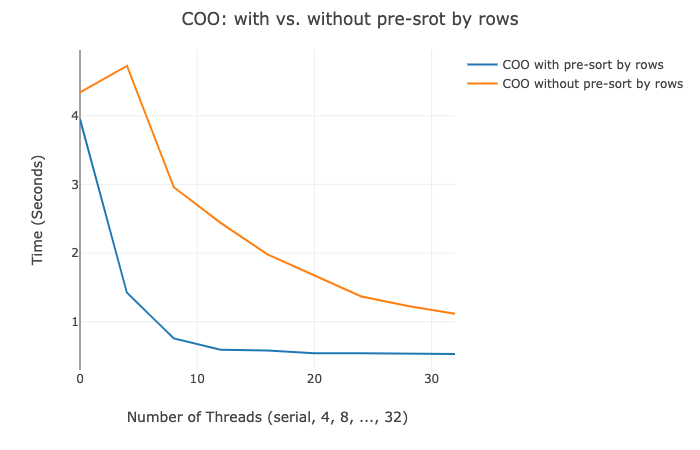
\includegraphics[scale=0.4]{./figures/coo_sort}
		\end{figure}

	\section{Findings}
		\begin{itemize}
			\item CSR needs to be pre-sorted by rows to be used for matrix multiplication. This is because, we need to sort rows to know row offsets, which is used to calculate row pointers.
			\item For sparse matrix multiplication (serial or parallel), CSR performs better than COO (with or without pre-sort by row).
			\item For parallelization, the number of threads affects CSR more than it affects COO.
			\item CSR's accuracy is not affected by the number of threads; COO's accuracy is affected when using more than 24 threads. However, the difference (\(10^{-10}\)) is acceptable and it is only for one or two elements.
			\item For COO format without pre-sort by rows, without lock, parallelization does not yield the correct result.
			\item For COO format without pre-sort by rows, but with lock, parallelization will yield result within \(10^{-10}\) difference.
			\item For COO format with pre-sort by rows, adding locks will hurt the performance. This is because once COO is pre-sorted by rows, adding locks is not needed.
		\end{itemize}
	
\end{document}